\documentclass[11pt]{book}
\usepackage{palatino}
\usepackage{amsfonts,amsmath,amssymb}
% \usepackage{graphicx}


\ifx\pdftexversion\undefined
    \usepackage[dvips]{graphicx}
\else
    \usepackage[pdftex]{graphicx}
    \usepackage{epstopdf}
    \epstopdfsetup{suffix=}
\fi


\begin{document}

%%%%%%%%%%%%%%%%%%%%%%%%%%%%%%%%%%%%%%%%
% Problem Set 3
%%%%%%%%%%%%%%%%%%%%%%%%%%%%%%%%%%%%%%%%

\pagestyle{empty}
{\noindent\bf Spring 2021 \hfill Firstname M.~Lastname}
\vskip 16pt
\centerline{\bf University of Central Florida}
\centerline{\bf College of Business}
\vskip 16pt
\centerline{\bf QMB 6911}
\centerline{\bf Capstone Project in Business Analytics}
\vskip 10pt
\centerline{\bf Solutions:  Problem Set \#3}
\vskip 32pt
\noindent


\section*{Summary Satistics}


\subsection*{Summary by Country of Manufacture}

% latex table generated in R 4.0.2 by xtable 1.8-4 package
% Thu Aug 06 16:21:59 2020
\begin{table}[ht]
\centering
\begin{tabular}{rlll}
  \hline
 & China & Korea & USA \\ 
  \hline
Min. Weight & 129.0 & 331.6 & 600.0 \\ 
  Mean Weight &  34.99 & 280.22 & 839.00 \\ 
  Max. Weight &  200.0 &  484.9 & 1095.0 \\ 
  Min. Diameter & 129.0 & 331.6 & 600.0 \\ 
  Mean Diameter &  34.99 & 280.22 & 839.00 \\ 
  Max. Diameter &  200.0 &  484.9 & 1095.0 \\ 
  Min. Width & 129.0 & 331.6 & 600.0 \\ 
  Mean Width &  34.99 & 280.22 & 839.00 \\ 
  Max. Width &  200.0 &  484.9 & 1095.0 \\ 
  Min. Price & 129.0 & 331.6 & 600.0 \\ 
  Mean Price &  34.99 & 280.22 & 839.00 \\ 
  Max. Price &  200.0 &  484.9 & 1095.0 \\ 
   \hline
\end{tabular}
\caption{Summary by Country of Manufacture} 
\label{tab:summ_by_country}
\end{table}



\clearpage
\subsection*{Country of Manufacture by Brand}

% latex table generated in R 4.0.5 by xtable 1.8-4 package
% Thu Jan 27 21:16:18 2022
\begin{table}[ht]
\centering
\begin{tabular}{rrrrr}
  \hline
 & China & Korea & USA & Total \\ 
  \hline
3-TAND & 15 & 0 & 0 & 15 \\ 
  Abel & 0 & 0 & 15 & 15 \\ 
  Allen & 0 & 18 & 7 & 25 \\ 
  Aspen & 0 & 0 & 8 & 8 \\ 
  Bauer & 0 & 0 & 2 & 2 \\ 
  Cheeky & 11 & 0 & 0 & 11 \\ 
  ECHO & 0 & 12 & 0 & 12 \\ 
  Galvan & 0 & 0 & 23 & 23 \\ 
  Hatch & 0 & 0 & 8 & 8 \\ 
  Loop & 0 & 14 & 0 & 14 \\ 
  Nautilus & 0 & 0 & 15 & 15 \\ 
  Orvis & 1 & 0 & 1 & 2 \\ 
  Ross & 0 & 0 & 28 & 28 \\ 
  Sage & 0 & 6 & 0 & 6 \\ 
  Taylor & 0 & 12 & 0 & 12 \\ 
  TFO & 0 & 16 & 0 & 16 \\ 
  Tibor & 0 & 0 & 4 & 4 \\ 
  Waterworks-Lamson & 0 & 8 & 24 & 32 \\ 
  Totals & 27 & 86 & 135 & 248 \\ 
   \hline
\end{tabular}
\caption{Country of Manufacture by Brand of Fly Reel} 
\label{tab:country_by_brand}
\end{table}



\clearpage
\subsection*{Reel Design by Brand of Fly Reel}

% latex table generated in R 4.0.5 by xtable 1.8-4 package
% Thu Jan 27 21:16:18 2022
\begin{table}[ht]
\centering
\begin{tabular}{rrrrrr}
  \hline
 & Unsealed & Sealed & Cast & Machined & Total \\ 
  \hline
3-TAND & 0 & 15 & 0 & 15 & 15 \\ 
  Abel & 9 & 6 & 0 & 15 & 15 \\ 
  Allen & 8 & 17 & 1 & 24 & 25 \\ 
  Aspen & 8 & 0 & 0 & 8 & 8 \\ 
  Bauer & 0 & 2 & 0 & 2 & 2 \\ 
  Cheeky & 6 & 5 & 6 & 5 & 11 \\ 
  ECHO & 9 & 3 & 12 & 0 & 12 \\ 
  Galvan & 20 & 3 & 0 & 23 & 23 \\ 
  Hatch & 0 & 8 & 0 & 8 & 8 \\ 
  Loop & 0 & 14 & 0 & 14 & 14 \\ 
  Nautilus & 4 & 11 & 0 & 15 & 15 \\ 
  Orvis & 0 & 2 & 0 & 2 & 2 \\ 
  Ross & 21 & 7 & 0 & 28 & 28 \\ 
  Sage & 2 & 4 & 0 & 6 & 6 \\ 
  Taylor & 0 & 12 & 0 & 12 & 12 \\ 
  TFO & 4 & 12 & 4 & 12 & 16 \\ 
  Tibor & 3 & 1 & 0 & 4 & 4 \\ 
  Waterworks-Lamson & 0 & 32 & 8 & 24 & 32 \\ 
  Totals & 94 & 154 & 31 & 217 & 248 \\ 
   \hline
\end{tabular}
\caption{Reel Design by Brand of Fly Reel} 
\label{tab:design_by_brand}
\end{table}



\clearpage
\subsection*{Categorical Variables by Country of Manufacture}

[To be added.]


%%%%%%%%%%%%%%%%%%%%%%%%%%%%%%%%%%%%%%%%
% Problem Set 4
%%%%%%%%%%%%%%%%%%%%%%%%%%%%%%%%%%%%%%%%

\pagebreak
\pagestyle{empty}
{\noindent\bf Spring 2021 \hfill Firstname M.~Lastname}
\vskip 16pt
\centerline{\bf University of Central Florida}
\centerline{\bf College of Business}
\vskip 16pt
\centerline{\bf QMB 6911}
\centerline{\bf Capstone Project in Business Analytics}
\vskip 10pt
\centerline{\bf Solutions:  Problem Set \#4}
\vskip 32pt
\noindent


\section*{Empirical Distribution Function of Fly Reel Prices}

\begin{figure}[h!]
  \centering
  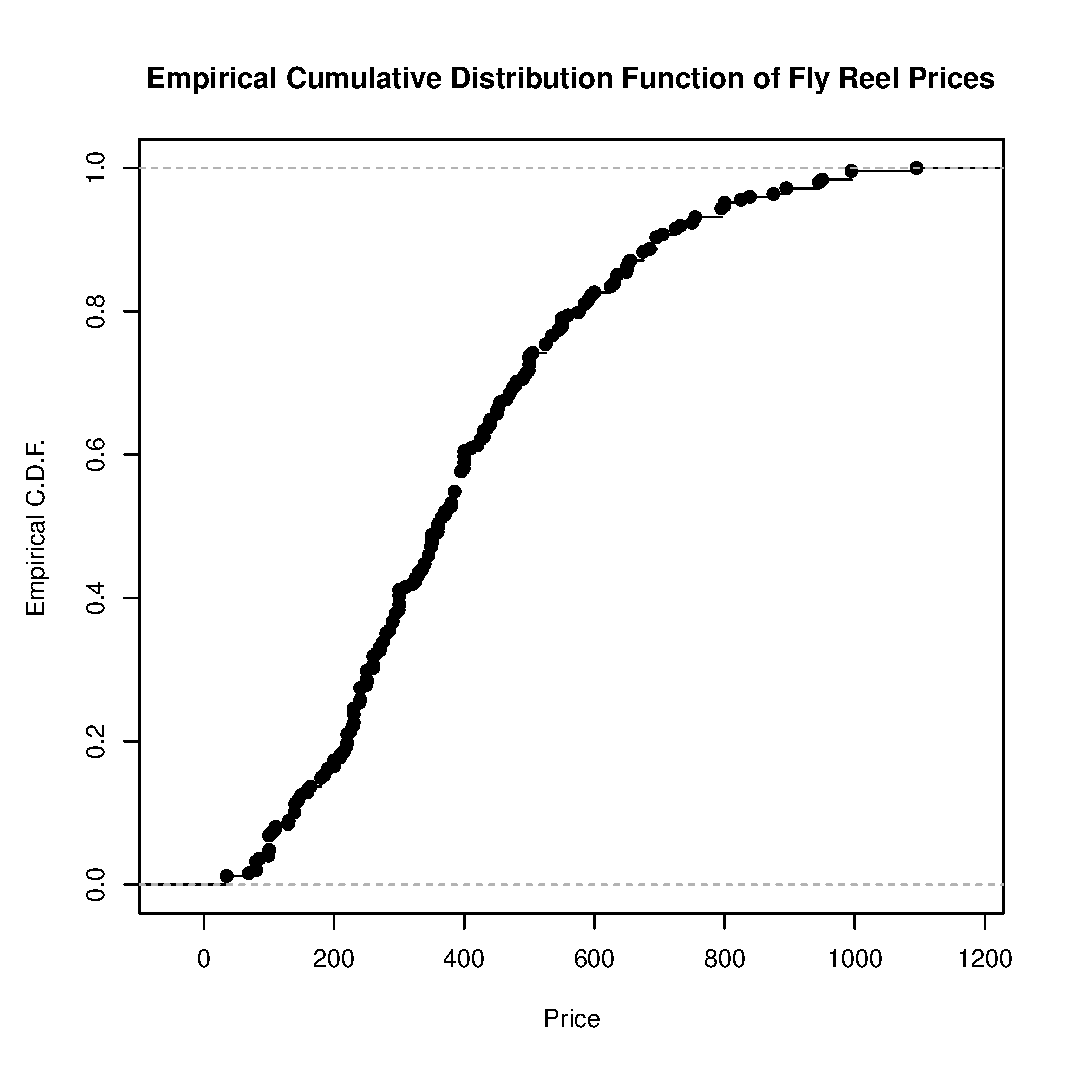
\includegraphics[scale = 0.5, keepaspectratio=true]{../Figures/ecdf_prices}
  \caption{Empirical Distribution Function of Fly Reel Prices} \label{fig:ecdf_prices}
\end{figure}


\section*{Relative Histogram of Fly Reel Prices}

\begin{figure}[h!]
  \centering
  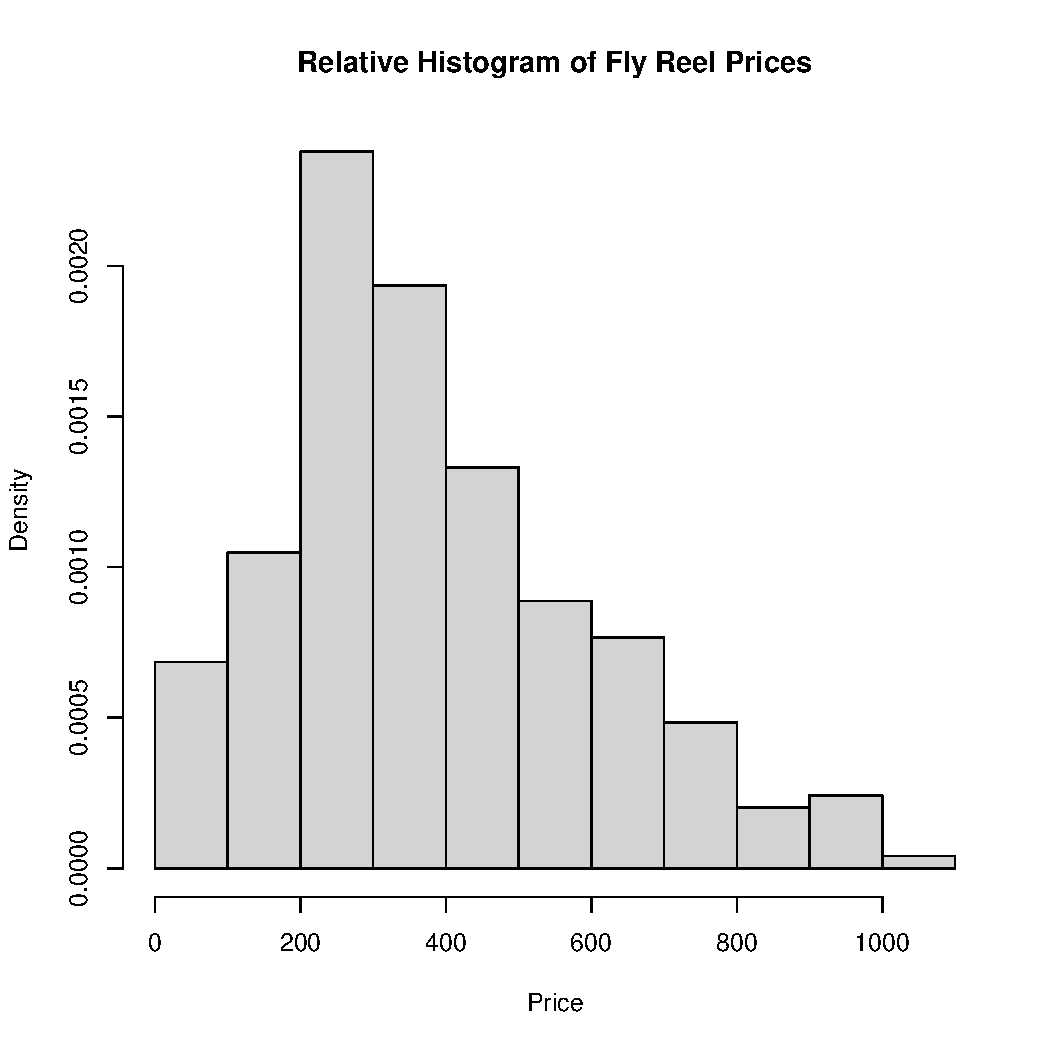
\includegraphics[scale = 0.5, keepaspectratio=true]{../Figures/hist_prices}
  \caption{Relative Histogram of Fly Reel Prices} \label{fig:hist_prices}
\end{figure}


\pagebreak
\section*{Probability Density Function of Fly Reel Prices}

This is the kernel-smoothed probability density function of the natural logarithm of
price:

\begin{figure}[h!]
  \centering
  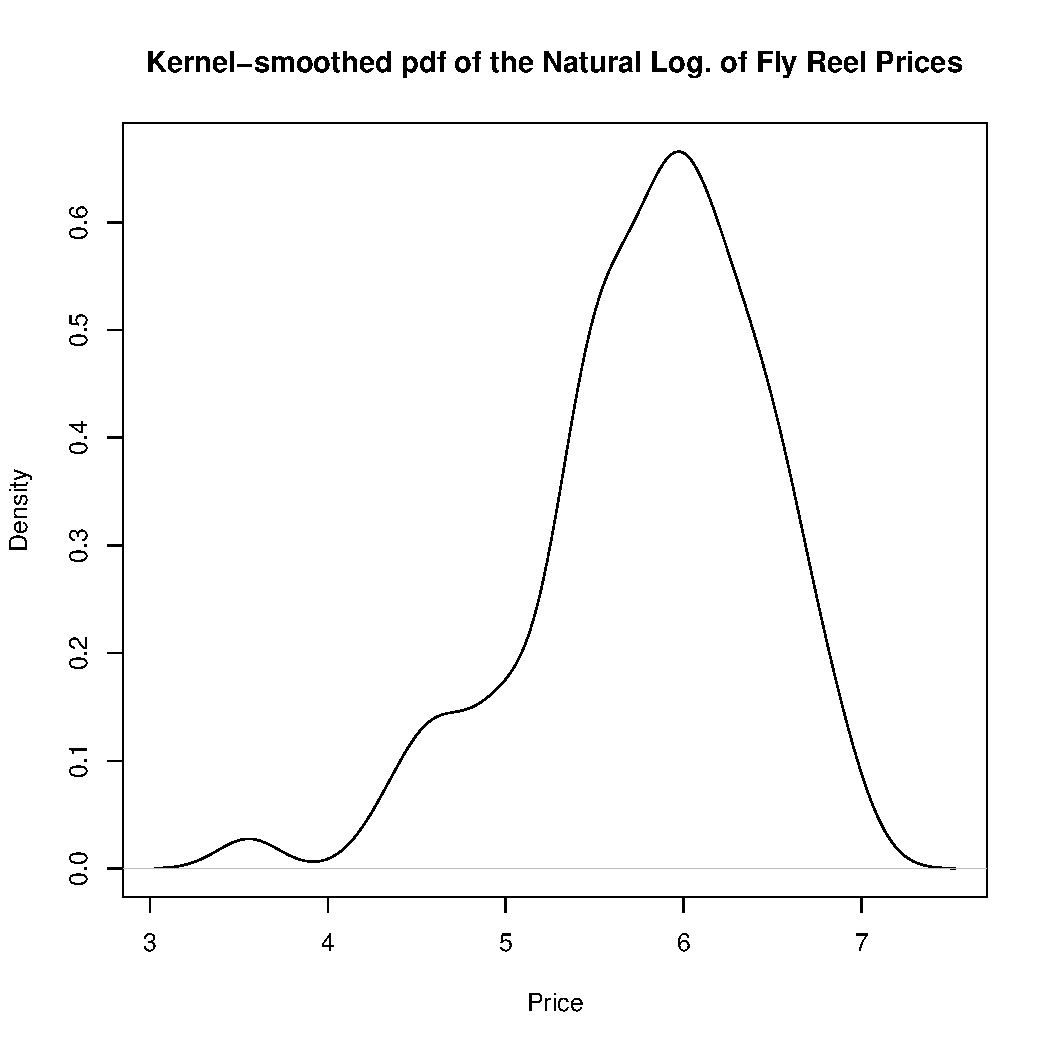
\includegraphics[scale = 0.5, keepaspectratio=true]{../Figures/density_prices}
  \caption{Probability Density Function of Fly Reel Prices} \label{fig:density_prices}
\end{figure}



%%%%%%%%%%%%%%%%%%%%%%%%%%%%%%%%%%%%%%%%
% Solution template
%%%%%%%%%%%%%%%%%%%%%%%%%%%%%%%%%%%%%%%%

\clearpage

\pagebreak
\pagestyle{empty}
{\noindent\bf Spring 2021 \hfill Firstname M.~Lastname}
\vskip 16pt
\centerline{\bf University of Central Florida}
\centerline{\bf College of Business}
\vskip 16pt
\centerline{\bf QMB 6911}
\centerline{\bf Capstone Project in Business Analytics}
\vskip 10pt
\centerline{\bf Solutions:  Problem Set \#x}
\vskip 32pt
\noindent
\begin{itemize}
\item[1.] Consider 

\begin{itemize}
\item[a)] Now

\item[b)] Then
\end{itemize}
\end{itemize}

%%%%%%%%%%%%%%%%%%%%%%%%%%%%%%%%%%%%%%%%
\end{document}
%%%%%%%%%%%%%%%%%%%%%%%%%%%%%%%%%%%%%%%%
